%\documentclass[9pt, xcolor=x11names,compress]{beamer}
\documentclass[9pt, xcolor={dvipsnames}]{beamer}
\usepackage{tabulary}
\usepackage{booktabs}
\usepackage{float}
\usepackage{graphicx}
\usepackage{mwe}% for example pictures
\usepackage{siunitx}
\usepackage{hyperref}
\usepackage[many]{tcolorbox}
\usepackage{multicol}

% >>> BOXES ==============================
\tcbset{
    sharp corners,
    colback = white,
    before skip = 0.2cm,    % add extra space before the box
    after skip = 0.5cm      % add extra space after the box
}    
\definecolor{main}{HTML}{e7e7e7}    
\definecolor{sub}{HTML}{F4F4F4}
\definecolor{sub2}{HTML}{f3f3f3}     
\newtcolorbox{boxH}{
    colback = sub, 
    colframe = main, 
    boxrule = 0pt, 
    leftrule = 6pt % left rule weight
}

% >>> COLORS =============================
\newcommand{\redline}[1]{\color{red}\uline{\textcolor{black}{#1}}\color{black}\:}
\newcommand{\ghl}[1]{\colorbox{sub2}{#1}\:}
\newcommand{\blue}[1]{\textcolor{blue}{#1}}
\newcommand{\red}[1]{\textcolor{BrickRed}{#1}}
\newcommand{\green}[1]{\textcolor{ForestGreen}{#1}}


% >>> BEAMER =============================
\definecolor{PRdark}{HTML}{00008B}
\definecolor{PRmedium}{HTML}{6082B6}
\definecolor{PRlight}{HTML}{B6D0E2}

\setbeamercolor*{structure}{bg=black,fg=PRdark}

\setbeamercolor*{palette primary}{use=structure,fg=white,bg=structure.fg!75!black}
\setbeamercolor*{palette secondary}{use=structure,fg=white,bg=structure.fg!50!black}
%\setbeamercolor*{palette secondary}{use=structure,fg=white,bg=structure.fg!75}
\setbeamercolor*{palette tertiary}{use=structure,fg=white, bg=structure.fg!50!black}
\setbeamercolor*{palette quaternary}{fg=white,bg=black}

\setbeamercolor{section in toc}{fg=black,bg=white}
\setbeamercolor{alerted text}{use=structure,fg=structure.fg!50!black!80!black}

\setbeamercolor{titlelike}{parent=palette primary,fg=structure.fg!50!black}
\setbeamercolor{frametitle}{bg=gray!15!white,fg=PRdark}

\setbeamercolor*{titlelike}{parent=palette primary}

% - 
\useoutertheme{infolines}
\usefonttheme[onlymath]{serif}

\setbeamertemplate{headline}[default]
\setbeamertemplate{navigation symbols}{}    %nav
\mode<beamer>{\setbeamertemplate{blocks}[shadow=false]}
\setbeamercovered{transparent}

\setbeamercolor{block body}{use=structure, fg=white, bg=black!20}
\setbeamercolor{itemize item}{fg=black}
\setbeamercolor{itemize subitem}{fg=gray} 
\setbeamercolor{itemize subsubitem}{fg=black!20} 

% >>> FOOTLINE ============================
\makeatletter
\setbeamertemplate{footline}
{  
\leavevmode%  
\hbox{%  

\begin{beamercolorbox}[wd=.333333\paperwidth,ht=2.25ex,dp=1ex,center]{author in head/foot}%    
\usebeamerfont{author in head/foot}
\insertshortauthor
\end{beamercolorbox}%  

\begin{beamercolorbox}[wd=0.666667\paperwidth,ht=2.25ex,dp=1ex,right]{date in head/foot}%    
\usebeamerfont{date in head/foot}\insertshortdate{}\hspace*{2em}    
\insertframenumber{} / \inserttotalframenumber\hspace*{2ex}  
\end{beamercolorbox}}%  

\vskip0pt%
}

\makeatother 
\useoutertheme[footline=empty, subsection=false]{miniframes}


% ===========================================
% ===========================================

\author{Pierre Rouillard}
\title{Soutenance Stage d'Application}
\institute{xx/xx/xxxx}
\date{\textit{Allianz Trade - ENSAE}} 

\begin{document}
\begin{frame}[plain]
\titlepage
\centering

\includegraphics[width=.5\textwidth]{Allianz_Trade.png}
\end{frame}

\section{Introduction}
\begin{frame}[label=Background]{Test1}
\begin{itemize}
\item Here to input your background\\
   \begin{itemize}
    \item This is the sub-content
    \item Here you can also jump to other slides \hyperlink{Rocky}{\beamergotobutton{}}
   \end{itemize}
\item Now we go back to the main content\\

\end{itemize}
\end{frame}

\section{Literature Review}
\begin{frame}{Here is the title of this slides}
\begin{boxH}
    $Y = X'.\widetilde{\beta} + \widetilde{\varepsilon}$ , $E[X\widetilde{\varepsilon}]=0$ \blue{toujours} définissable sous conditions de moments.
\end{boxH}
\end{frame}

\section{Method}
\begin{frame}[label=Rocky]{There you can also separate the page}
\begin{figure}
 \begin{columns}[c]
  \begin{column}{0.3\textwidth}
    \centering
    
\includegraphics[width=1\textwidth]{Figure2.jpg}
  \end{column}
  \begin{column}{0.3\textwidth}
    \centering
    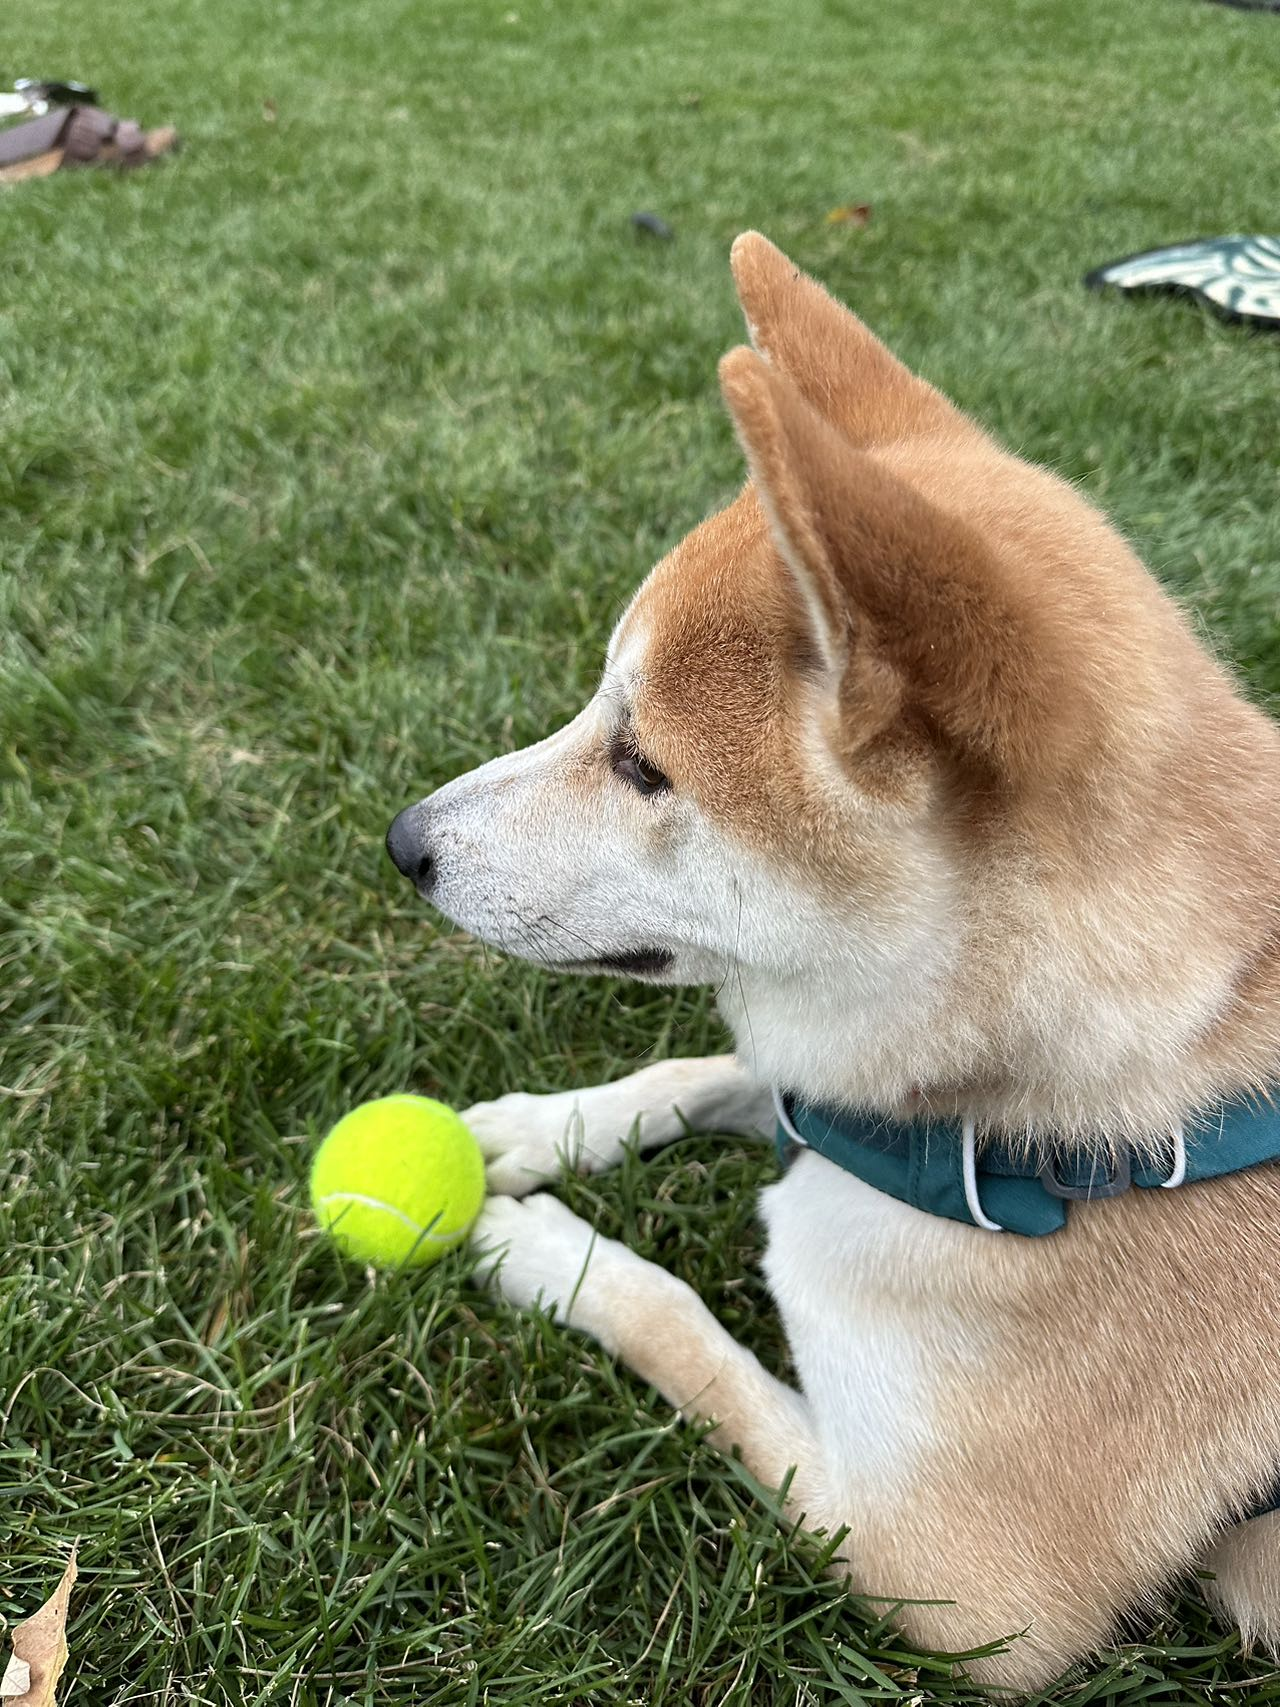
\includegraphics[width=1\textwidth]{Figure3.jpg}
  \end{column}
  \end{columns}
  \caption{Here I just using one caption for these 2 cute pictures but you can also using 2 captions  \parbox{\linewidth}{\small\textit{Data source: Rocky's daily look}}}
\end{figure}
Now I am going back to the previous slidesby clicking this: \hyperlink{Background}{go back}
\end{frame}

\section{Results}
\begin{frame}{Results}
\input{table_Results}
\end{frame}

\begin{frame}
 \begin{center}
		{\Huge Merci!}\\
		\bigskip\bigskip % Vertical whitespace
		{\LARGE pierre.rouillard@ensae.fr}
	\end{center}
\end{frame}

\end{document}